\def\year{2021}\relax
%File: formatting-instructions-latex-2021.tex
%release 2021.2
\documentclass[letterpaper]{article} % DO NOT CHANGE THIS
\usepackage{aaai21}  % DO NOT CHANGE THIS
\usepackage{times}  % DO NOT CHANGE THIS
\usepackage{helvet} % DO NOT CHANGE THIS
\usepackage{courier}  % DO NOT CHANGE THIS
\usepackage[hyphens]{url}  % DO NOT CHANGE THIS
\usepackage{graphicx} % DO NOT CHANGE THIS
\urlstyle{rm} % DO NOT CHANGE THIS
\def\UrlFont{\rm}  % DO NOT CHANGE THIS
\usepackage{natbib}  % DO NOT CHANGE THIS AND DO NOT ADD ANY OPTIONS TO IT
\usepackage{caption} % DO NOT CHANGE THIS AND DO NOT ADD ANY OPTIONS TO IT
\frenchspacing  % DO NOT CHANGE THIS
\setlength{\pdfpagewidth}{8.5in}  % DO NOT CHANGE THIS
\setlength{\pdfpageheight}{11in}  % DO NOT CHANGE THIS
%\nocopyright
%PDF Info Is REQUIRED.
% For /Author, add all authors within the parentheses, separated by commas. No accents or commands.
% For /Title, add Title in Mixed Case. No accents or commands. Retain the parentheses.
\pdfinfo{
/Title (AAAI Press Formatting Instructions for Authors Using LaTeX -- A Guide)
/Author (AAAI Press Staff, Pater Patel Schneider, Sunil Issar, J. Scott Penberthy, George Ferguson, Hans Guesgen, Francisco Cruz, Marc Pujol-Gonzalez)
/TemplateVersion (2021.2)
} %Leave this
% /Title ()
% Put your actual complete title (no codes, scripts, shortcuts, or LaTeX commands) within the parentheses in mixed case
% Leave the space between \Title and the beginning parenthesis alone
% /Author ()
% Put your actual complete list of authors (no codes, scripts, shortcuts, or LaTeX commands) within the parentheses in mixed case.
% Each author should be only by a comma. If the name contains accents, remove them. If there are any LaTeX commands,
% remove them.

% DISALLOWED PACKAGES
% \usepackage{authblk} -- This package is specifically forbidden
% \usepackage{balance} -- This package is specifically forbidden
% \usepackage{color (if used in text)
% \usepackage{CJK} -- This package is specifically forbidden
% \usepackage{float} -- This package is specifically forbidden
% \usepackage{flushend} -- This package is specifically forbidden
% \usepackage{fontenc} -- This package is specifically forbidden
% \usepackage{fullpage} -- This package is specifically forbidden
% \usepackage{geometry} -- This package is specifically forbidden
% \usepackage{grffile} -- This package is specifically forbidden
% \usepackage{hyperref} -- This package is specifically forbidden
% \usepackage{navigator} -- This package is specifically forbidden
% (or any other package that embeds links such as navigator or hyperref)
% \indentfirst} -- This package is specifically forbidden
% \layout} -- This package is specifically forbidden
% \multicol} -- This package is specifically forbidden
% \nameref} -- This package is specifically forbidden
% \usepackage{savetrees} -- This package is specifically forbidden
% \usepackage{setspace} -- This package is specifically forbidden
% \usepackage{stfloats} -- This package is specifically forbidden
% \usepackage{tabu} -- This package is specifically forbidden
% \usepackage{titlesec} -- This package is specifically forbidden
% \usepackage{tocbibind} -- This package is specifically forbidden
% \usepackage{ulem} -- This package is specifically forbidden
% \usepackage{wrapfig} -- This package is specifically forbidden
% DISALLOWED COMMANDS
% \nocopyright -- Your paper will not be published if you use this command
% \addtolength -- This command may not be used
% \balance -- This command may not be used
% \baselinestretch -- Your paper will not be published if you use this command
% \clearpage -- No page breaks of any kind may be used for the final version of your paper
% \columnsep -- This command may not be used
% \newpage -- No page breaks of any kind may be used for the final version of your paper
% \pagebreak -- No page breaks of any kind may be used for the final version of your paperr
% \pagestyle -- This command may not be used
% \tiny -- This is not an acceptable font size.
% \vspace{- -- No negative value may be used in proximity of a caption, figure, table, section, subsection, subsubsection, or reference
% \vskip{- -- No negative value may be used to alter spacing above or below a caption, figure, table, section, subsection, subsubsection, or reference

\setcounter{secnumdepth}{0} %May be changed to 1 or 2 if section numbers are desired.

\usepackage{siunitx}
\usepackage[dvipsnames]{xcolor}
\newcommand{\todo}[1]{\textcolor{blue}{#1}}

% The file aaai21.sty is the style file for AAAI Press
% proceedings, working notes, and technical reports.
%

% Title

% Your title must be in mixed case, not sentence case.
% That means all verbs (including short verbs like be, is, using,and go),
% nouns, adverbs, adjectives should be capitalized, including both words in hyphenated terms, while
% articles, conjunctions, and prepositions are lower case unless they
% directly follow a colon or long dash
\iffalse
\title{AAAI Press Formatting Instructions \\for Authors Using \LaTeX{} --- A Guide }
\author{
    %Authors
    % All authors must be in the same font size and format.
    Written by AAAI Press Staff\textsuperscript{\rm 1}\thanks{With help from the AAAI Publications Committee.}\\
    AAAI Style Contributions by Pater Patel Schneider,
    Sunil Issar,  \\
    J. Scott Penberthy,
    George Ferguson,
    Hans Guesgen,
    Francisco Cruz,
    Marc Pujol-Gonzalez
    \\
}
\affiliations{
    %Afiliations
    \textsuperscript{\rm 1}Association for the Advancement of Artificial Intelligence\\
    %If you have multiple authors and multiple affiliations
    % use superscripts in text and roman font to identify them.
    %For example,

    % Sunil Issar, \textsuperscript{\rm 2}
    % J. Scott Penberthy, \textsuperscript{\rm 3}
    % George Ferguson,\textsuperscript{\rm 4}
    % Hans Guesgen, \textsuperscript{\rm 5}.
    % Note that the comma should be placed BEFORE the superscript for optimum readability

    2275 East Bayshore Road, Suite 160\\
    Palo Alto, California 94303\\
    % email address must be in roman text type, not monospace or sans serif
    publications21@aaai.org

    % See more examples next
}
\fi
\iffalse
%Example, Single Author, ->> remove \iffalse,\fi and place them surrounding AAAI title to use it
\title{My Publication Title --- Single Author}
\author {
    % Author
    Author Name \\
}

\affiliations{
    Affiliation \\
    Affiliation Line 2 \\
    name@example.com
}
\fi


%Example, Multiple Authors, ->> remove \iffalse,\fi and place them surrounding AAAI title to use it
\title{Domain-agnostic Outlier Ranking Algorithms (DORA)---A Configurable Pipeline for Facilitating Outlier Detection in Scientific Datasets}
\author {
    % Authors
    First Author Name,\textsuperscript{\rm 1}
    Second Author Name, \textsuperscript{\rm 2}
    Third Author Name \textsuperscript{\rm 1} \\
}
\affiliations {
    % Affiliations
    \textsuperscript{\rm 1} Affiliation 1 \\
    \textsuperscript{\rm 2} Affiliation 2 \\
    firstAuthor@affiliation1.com, secondAuthor@affilation2.com, thirdAuthor@affiliation1.com
}

\begin{document}

\maketitle

\begin{abstract}
Automatic detection of out-of-distribution (OOD) samples or features is
universally needed when working with scientific datasets. For example,
OOD detection methods can be used for cleaning datasets or flagging
novel samples in order to guide instrument acquisition or scientific analysis.
We present Domain-agnostic Outlier Ranking Algorithms (DORA) to provide
a configurable pipeline that makes it easy for scientists to apply and evaluate
outlier detection methods in a variety of domains. DORA allows users to 
configure outlier detection experiments by specifying the location of their 
dataset(s), the input data type, feature extraction methods, and which 
algorithms should be applied. DORA supports image, raster, time series, 
or feature vector input data types and outlier detection methods that include
 Isolation Forest, Discovery via Eigenbasis Modeling of Uninteresting Data 
 (DEMUD), principal component analysis (PCA), Reed-Xiaoli (RX) detector, 
 Local RX, negative sampling, and probabilistic autoencoder. Given a set of
  data samples, each algorithm assigns an outlier score to each sample. DORA
   provides results organization and visualization modules to help users 
   process the results, including sorting samples by outlier score, evaluating 
   outlier recall for a set of known/labeled outliers, clustering groups of 
   similar outliers together, and causal graphs. To demonstrate the 
   cross-domain applicability of DORA, we conducted outlier detection
    experiments for three real-world use cases: 1) cleaning noisy ground-truth 
    datasets (Earth Science), 
     2) flagging non-astrophysical objects in the Dark Energy Survey 
     (astrophysics), and 3) novelty-guided onboard targeting of instruments
      for Mars rovers (planetary science). [We showed that ...]
\end{abstract}

\section{Introduction}
The ability to automatically detect out-of-distribution samples in large data 
sets is of interest for a wide variety of scientific domains. Depending on the
 application setting, this capability is also commonly referred to as anomaly
  detection, outlier detection, or novelty detection. More broadly, this is 
  referred to as out-of-distribution (OOD) detection. In general, the goal of 
  OOD detection systems is to identify samples that deviate from the majority
   of samples in a dataset in an unsupervised manner (Pimentel et al., 2014). 
   In machine learning, these methods are commonly used for identifying 
   mislabeled or otherwise invalid samples in a dataset 
   (e.g., Liang et al., 2018; Böhm et al., 2020). 
   
   When working with science datasets, OOD detection can be used for 
   cleaning datasets, e.g., flagging ground-truth labels with GPS or human
    entry error or identifying wrongly categorized objects in a catalog. 
    It could also be used for discovery, e.g., to flag novel samples in order 
    to guide instrument acquisition or scientific analysis. Another application
   is the detection of rare objects that are known to exist but the known
   examples are too few to create a large enough labeled dataset for 
   supervised classification algorithms. 
  Despite wide differences in applications, data types, and dimensionality,
 the same underlying machine learning algorithms can be employed across 
 all of these domains. A challenge for applying them however is that domain
 scientists do not always have the programming or machine learning background
 to apply the algorithms themselves using existing tools. Given the widespread 
 applicability and transferability of OOD methods, the scientific community 
 would benefit from a tool that made it easy for them to apply popular outlier
 detection algorithms to their science datasets. We created DORA (Domain-
 agnostic Outlier Ranking Algorithms) to provide a tool for applying outlier 
 detection algorithms to a variety of scientific data sets with minimal coding
 required. Users need only to specify details for their data/application 
 including the data type, location, and algorithms to run in an experiment
 configuration file. DORA supports image, raster, time series, 
or feature vector input data types and outlier detection methods that include
 Isolation Forest, Discovery via Eigenbasis Modeling of Uninteresting Data 
 (DEMUD)~\citep{wagstaff:demud13}, principal component analysis (PCA),
   Reed-Xiaoli (RX) detector,  
 Local RX, negative sampling~\cite{sipple:neg-sampling20}, and probabilistic 
 autoencoder. Given a set of data samples, each algorithm assigns an outlier 
 score to each sample. DORA provides results organization and visualization 
 modules to help users process the results, including sorting samples by outlier 
 score, evaluating outlier recall for a set of known/labeled outliers, clustering 
 groups of similar outliers together, and causal graphs. To demonstrate the 
 cross-domain applicability of DORA, we conducted outlier detection experiments 
 for three real-world use cases: 1) cleaning noisy ground-truth datasets (Earth 
 Science), 2) flagging non-astrophysical objects in the Dark Energy Survey 
 (astrophysics), and 3) novelty-guided onboard targeting of instruments for Mars 
 rovers (planetary science). \todo{[We showed that ...]}

\section{Related Work}
In astrophysics, 
    outlier detection methods have been employed for identifying astrophysical
     objects with unique characteristics (Xiong et al., 2010; 
     Storey-Fisher et al., 2020; Hayat et al., 2020) as well as 
     data/modeling artifacts~\citep{wagstaff:des-anom20} (Lochner et al., 2020) in 
     astronomical surveys. Examples of outlier detection applications in 
     Earth science include detecting anomalous objects or materials 
     (Chang and Chiang, 2002; Zhou et al., 2016), data artifacts/noise 
     (Liu et al., 2017; Alvera-Azcárate et al., 2012), change (Touati et al.,
      2020; Zhou et al., 2016),  and ocean extremes (Prochaska et al.). 
      Planetary science applications of outlier detection have mostly focused 
      on prioritizing samples with novel geologic or geochemical features for
       follow-up targeting or analysis (Kerner et al., 2020a; Kerner et al., 
       2020b) \citep{wagstaff:demud13}.

\begin{itemize}
\item Methods for outlier detection
\item Applications of outlier detection related to our focus domains 
(e.g., \citet{kerner2020comparison})
\item Outlier detection toolkits: PyOD Python
package~\citep{zhao:pyod19}, \url{https://github.com/yzhao062/pyod} 
\item Tools for applying outlier detection or other methods across
domains?
\end{itemize}

\section{Methods}

%\subsection{DORA configurable pipeline} 
Figure \ref{fig:dora} illustrates the architecture of DORA. It includes 
data loading, feature extraction, outlier ranking, results organization, and 
results visualizaiton modules. The DORA pipeline is implemented in Python 3.
In order to improve the readability and execution speed of the code, we adopted
object-oriented and functional programming practices.  We designed DORA to be 
readily extensible to support additional data types or formats, outlier detection 
algorithms, and results organization or visualization methods by writing new 
modules that follow the DORA API. Experimental settings are controlled by 
configuration files. In a configuration file, users can specify the input data, 
feature extraction methods, normalization method, outlier ranking methods, and 
results organization methods. 

\paragraph{Data types.} We chose to initially implement data loaders for four
data types that are commonly used by the machine learning and domain science
communities: time series, feature vectors, images (grayscale or RGB), and 
$N$-band rasters. $N$-band rasters are essentially images in which every pixel
is associated with a location defined by a geographic coordinate reference 
system (e.g., latitude/longitude in degrees). Most satellite data are 
distributed as rasters; common formats include GeoTIFF, NetCDF, and 
HDF. A data loader for each data type locates the data by the path(s)
defined in the configuration file and loads samples into a dictionary of numpy
 arrays indexed by the sample id. This \texttt{data\_dict} is then passed to each of the ranking algorithms specified in 
 the configuration file.

\paragraph{Outlier ranking algorithms.} We implemented 7 algorithms for 
scoring and 
ranking samples by outlierness. All algorithms are unsupervised.
We chose these algorithms to include a diverse
set of approaches to scoring outliers since different algorithms may have 
better performance for different datasets and use cases. 
%We describe each
%approach to scoring outliers and the associated methods below.

\begin{figure}
    \centering
    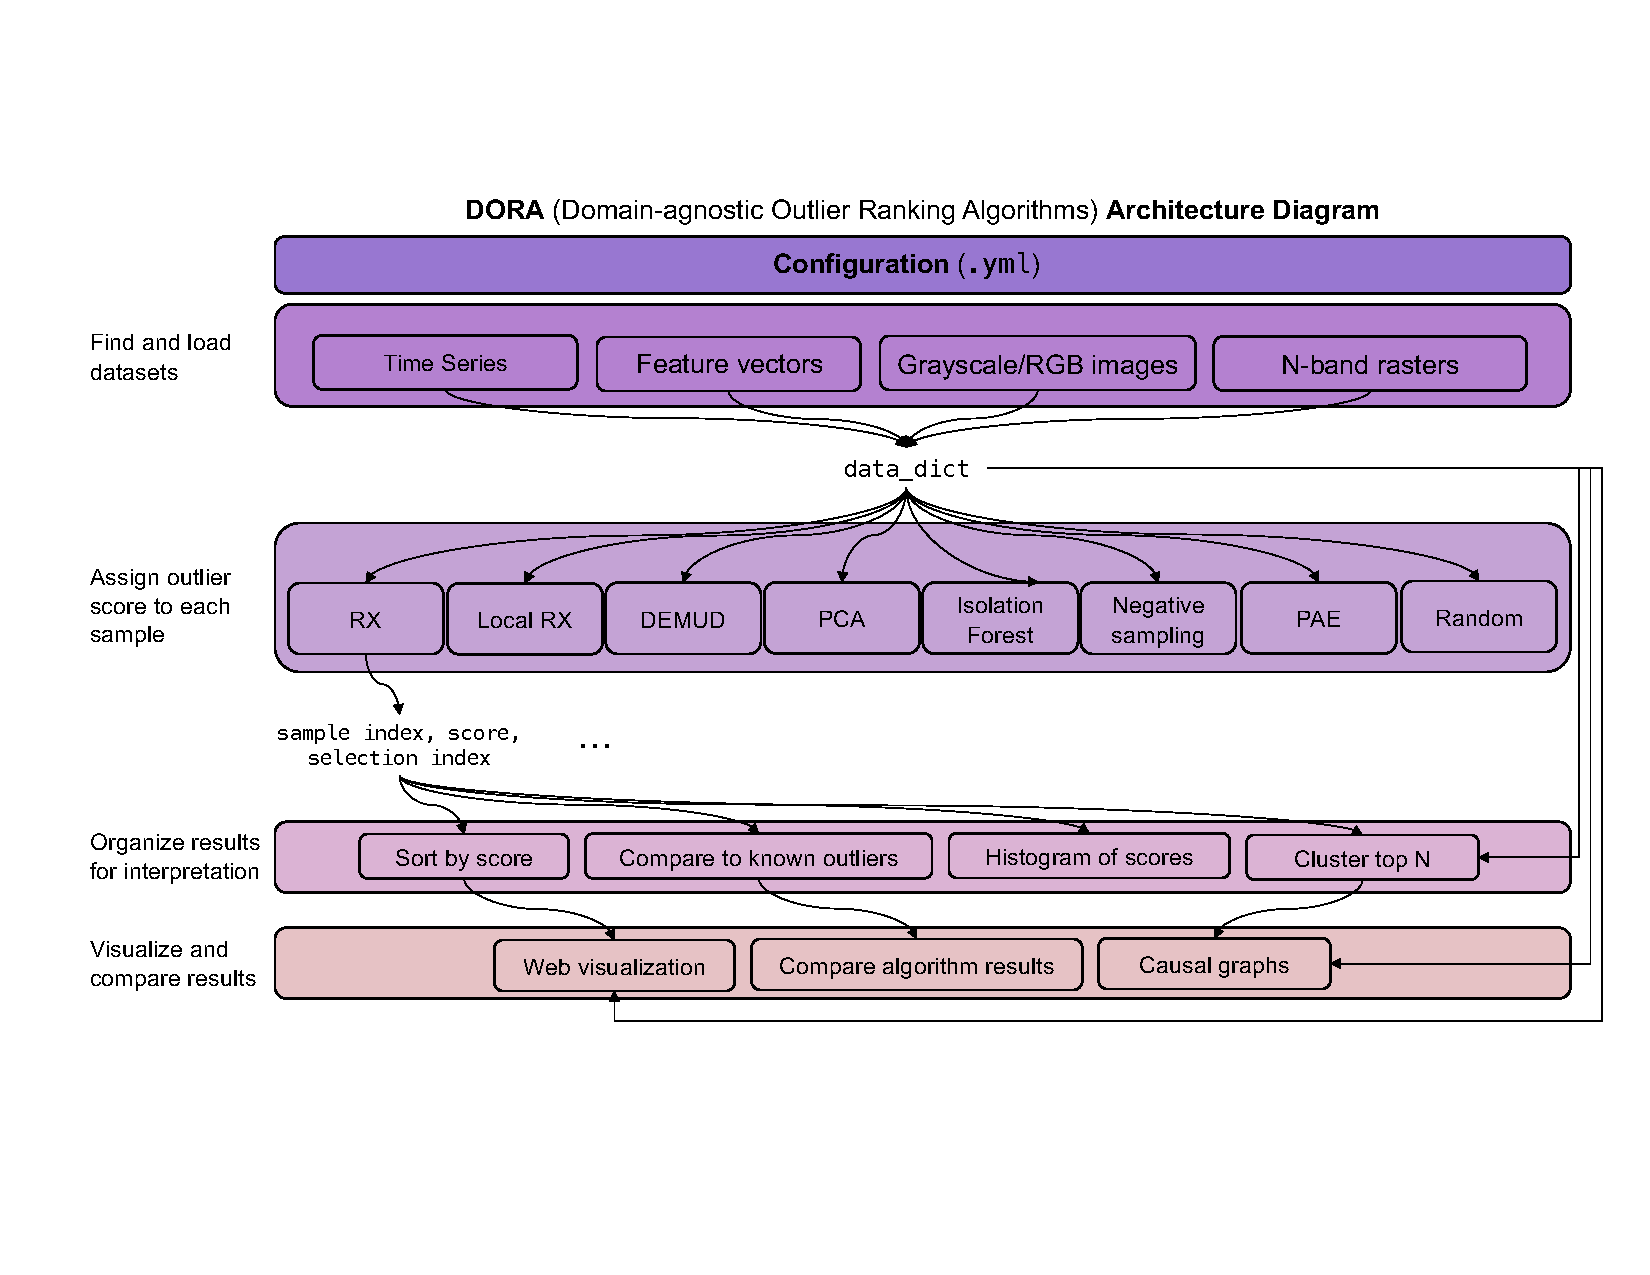
\includegraphics[width=\linewidth]{figures/dora-system-diagram-v5.pdf}
    \caption{DORA pipeline architecture.}
    \label{fig:dora}
\end{figure}

\subparagraph{Reconstruction error.}
Reconstruction-based methods aim to construct a model of a dataset by learning 
a mapping between the data samples and a lower-dimensional representation that
 minimizes the loss between the input and its reconstruction from the 
 low-dimensional representation~\citep{kerner2020comparison}. The 
 reconstruction error is used to compute the outlier score because samples
  that are unlike the data used to fit the model will be more poorly 
  reconstructed compared to inliers. 
Principal component analysis (PCA) has been used for outlier detection by
scoring samples using the reconstruction error (here, the L2 norm)
between inputs and their inverse
 transformation from the principal subspace~\citep{kerner2020comparison}.
The DEMUD algorithm~\citep{wagstaff:demud13} differs from other
outlier ranking methods: instead of independently scoring all
observations, DEMUD incrementally identifies the most unusual
remaining item, then incorporates it into the model of ``known''
(non-outlier) observations before selecting the next most unusual
item.  DEMUD's goal is to identify diverse outliers and avoid
redundant selections.  Once an outlier is encountered, repeated
occurrences of that outlier are deprioritized.  Methods that score
outliers independently maximize coverage of outliers, while DEMUD
maximizes the fast discovery of distinct outlier types.

\subparagraph{Distance.}
Distance-based methods score outliers based on their distance from some
``background'' which is usually defined by a sample distribution. The 
Reed-Xiaoli (RX) detector is commonly used for anomaly detection in
multispectral and hyperspectral remote sensing; RX uses the Mahalanobis
 distance between a sample and a background dataset mean and covariance
 to score samples~\citep{reed1990adaptive}. The local variant of RX (Local
 RX or LRX) can be used for image or raster data types and scores each pixel in
  an image with respect to a window ``ring'' of pixels surrounding 
  it~\citep{molero2013analysis}. 
  LRX requires two parameters that define the ring: an outer window which 
  defines the size of the window surrounding the pixel and an inner window
   which defines the size of the window around the target pixel to exclude from
   the background distribution. 

\subparagraph{Sparsity.}
Sparsity-based methods score outliers based on how isolated or sparse they
are in the feature space. Isolation forests are a common sparsity-based method
that constructs many random binary trees from a 
dataset~\cite{liu2008isolation}. The outlier score for
a sample is quantified as the average distance from the root to the item’s 
leaf. Shorter distances are indicative of outliers because fewer splits were 
required to isolate the sample.

\subparagraph{Probability.}
The negative sampling algorithm is implemented by converting the unsupervised 
outlier ranking problem into a semi-supervised 
problem~\citep{sipple:neg-sampling20}. Negative (anomalous) 
examples are created by sampling from an expanded space defined by the minimum 
and maximum values of each dimension of the positive (normal) examples. The 
negative and positive examples are then used to train a random forest 
classifier. We use the posterior probabilities of the random forest classifier 
as outlier scores, which means that the observations with higher posterior 
probabilities are more likely to be outliers.
The probabilistic autoencoder is a generative model consisting of an
autoencoder trained to reconstruct input data which is interpreted
probabilistically after training using a normalizing flow on the autoencoder
latent space~\cite{bohm2020probabilistic}.
Samples are scored as outliers using the log likelihood in the latent
distribution, the autoencoder reconstruction error, or a combination of
both.

\paragraph{Results organization.} 
Each of the outlier ranking algorithms returns an array containing the sample
index, outlier score, and selection index (index of each sample after sorting
by outlier score). DORA provides results organization modules intended to help
 users interpret and make decisions based on these outputs. The simplest 
 module saves a CSV of the samples sorted by their outlier score 
 (i.e., selection order). Clustering the top
  $N$ outlier selections can enable users to investigate the different types of 
 outliers that might be present in the dataset; this could be especially useful
 for separating outliers caused by noise or data artifacts vs. scientifically 
 interesting samples. We implemented the K-means and self-organizing maps 
 (SOMs) algorithms for clustering the top-N outliers. For use cases in which an
 evaluation dataset containing known outliers is available, we provide a module
 to assess how well algorithm selections correlate with known outliers. This is
 done by plotting the number of true outliers vs. number of selections made. 
  Finally,
 we provide a module for plotting histograms of outlier scores to visualize the
 distribution of scores in the dataset (which may be, e.g., multimodal or 
 long-tailed).

\paragraph{Results visualization.} 
\todo{Jake: describe website if ready by deadline.}
\todo{Eric: describe causal graphs if added by deadline.}

\section{Datasets}

We constructed three datasets to evaluate the utility of DORA and the
performance of each ranking algorithm for a variety of scientific domains
 (astrophysics, planetary science, and Earth science). We also included a 
 benchmark dataset that uses MNIST and Fashion-MNIST. Table \ref{tab:datasets}
 summarizes the number of unlabeled samples used for training and labeled
 samples used for evaluation for each dataset. We describe each in detail
 below.

\subsubsection{Astrophysical objects in Dark Energy Survey.}
\todo{Umaa}

\subsubsection{Targets in Mars rover images.}
Mars exploration is fundamentally an exercise in discovery with the
goal of increasing our understanding of the history, evolution,
composition, and currently active processes on Mars.  Outliers
identified in Mars observations can inspire new discoveries and inform
the choice of which areas merit follow-up or deeper
investigation~\cite{kerner2020comparison,wagstaff:rover-novelty20}.
We collected \num{72} images from the Navigation camera (Navcam) 
on the Mars Science Laboratory (MSL) rover
and employed the Rockster~\cite{burl:rockster16}
method currently used by onboard rover software to identify candidate rock
targets with an area of at least 100 pixels, yielding \num{1050}
targets.  We cropped out a \num{64}$\times$\num{64} pixel image
centered on each target.

We simulated the operational setting in which the rover has observed
targets up through mission day (sol) $s$ and the goal is to rank all
subsequent targets (after sol $s$) to inform which recent targets
merit further study.  Our rover image data covers sols \num{1343}
to \num{1703}.  We partitioned the images chronologically to assess
outlier detection in the 10 most recent sols, using ``prior'' set
$D_{1343-1693}$ ($n=992$) and ``assessment'' set $D_{1694-1703}$
($n=58)$ for evaluation.

We collaborated with an MSL science planning team member to
independently review the targets in $D_{1694-1703}$ and identify those
that were 
considered novel by the mission ($n_{outlier} = 9$).  Our goal for
this application is to assess how well the selections made by each
algorithm correlate with human novelty judgments to determine which
methods would be most suitable for informing onboard decisions about
follow-up observations.

\subsubsection{Satellite time series for ground-truth observations.}
Many Earth science applications using satellite Earth observation (EO) data
 require ground-truth observations for understanding and modeling ground-
 identified objects in the satellite observations. These ground observations
 also serve as labels that are paired with satellite data inputs for machine 
 learning models. For example, a model trained to classify crop types in
 satellite observations requires geo-referenced labels of crop type annotated
 in the field~\cite{tseng2021learning}. A widespread challenge of using ground-
 annotated datasets is that there are often points with erroneous location or 
 label information (e.g., due to GPS location error or human entry error) that
 need to be cleaned before the dataset can be used for machine learning or
 other downstream use cases. Automatically detecting these outliers could save 
 substantial time required for cleaning datasets and improve the performance of
 downstream analyses that rely on high-quality datasets. 
 %
 We used a dataset of ground
 observations of fall army worm (FAW) in maize crops collected by the UN Food
 and Agriculture Organization (FAO). This dataset includes 6,757 samples
 with location (latitude/longitude) metadata primarily in Africa and Southeast
 Asia. Most locations coincide with crop
 fields but there are many outliers that coincide with other land cover types 
 such as water, buildings, or forests. We constructed an evaluation set 
 consisting of all samples in Kenya ($n=113$) and manually annotated whether 
 each sample was considered an inlier (i.e., located in a crop field) or not 
 using high-resolution Planet satellite images in Collect Earth 
 Online~\cite{planetdata} ($n_{inlier}=76$, $n_{outlier}=37$). We used Google
 Earth Engine to export the Sentinel-1 synthetic aperture radar (SAR) monthly
 time series for each sample location, using data from year each sample was 
 collected. We used SAR data because it is sensitive to ground texture and
  penetrates clouds, which is important for the often-cloudy region covered
  by the dataset. Our goal for this application is to assess how well the 
  selections made by each algorithm correlate with outliers determined by
  visual inspection of the satellite images.
% descoped for lack of time and space
% \todo{If we have time, I want to also evaluate the downstream classifier
% performance before and after removing top N outliers with DORA.}

% Decided to cut this use case to make the presentation simpler (only one
% Earth science use case, and we already have a 1-band image dataset
% (Navcam). 
%\subsubsection{Volcanic thermal anomalies}

\subsubsection{MNIST and Fashion-MNIST.}
We included MNIST and F-MNIST to demonstrate the capabilities of DORA with a
traditional benchmark dataset. We used 60,000 images from 
F-MNIST as the training set and a combined set of 2,000 images from MNIST and 
F-MNIST as the evaluation set. Well-discriminating algorithms should assign 
higher outlier scores to samples from MNIST than F-MNIST.

\begin{table}
  \caption{Number of samples in the training and test sets for each dataset.}
  \label{tab:datasets}
  \centering
  \begin{tabular}{l|c|cc}
    \hline
    Dataset & Training & \multicolumn{2}{c}{Test}\\
     & Unlabeled &  Outliers &  Inliers \\
    
    \hline
    Astrophysics &   &   &   \\
    Earth & 6,757 & 37 & 76  \\
    Planetary & 992 &  9 & 49 \\
    F-MNIST & 60,000 & 1,000 & 1,000  \\
    \hline
  \end{tabular}
\end{table}

\section{Results}
The experimental setup for each dataset was to fit or train a model for
each ranking algorithm using a larger unlabeled dataset and then apply 
the models to compute the outlier scores for a smaller test dataset for which
labels of known outliers were available (Table \ref{tab:datasets}). 
For each test set, we created a plot of the number of known/true outliers 
detected out of the top $N$ selections. We also 
reported the Mean Discovery Rate (MDR) in the legend
for each algorithm to give a quantitative comparison of the curves that could
be comparable across the datasets. We defined MDR as:
\begin{equation}
MDR = \frac{\sum^{N_s}_{i=1} n_i}{\sum^{N_s}_{i=1} s_i}
\end{equation}
where $i \in [1, N_s]$ is the selection index,
 $N_s$ is the total number of selections,
 $s_i$ is the number of selections made up to index $i$,
 and $n_i$ is the number of known outliers (true positives)
among $s_i$ selections.
We also reported the precision at $N=n_{outlier}$ for each test set where
$n_{outlier}$ is the number of known outliers, i.e.,  the precision obtained 
when the number of selections is the same as the total number of outliers. 
Precision at $N$ is the number of true outliers divided by the number of 
selections $N$~\citep{campos2016evaluation}.
Table~\ref{tab:faw_results} compares the precision at $N=n_{outlier}$ for
each dataset and ranking algorithm. 
\todo{Jake: add description of theoretical random baseline.}
%\todo{Hannah: Consider merging all three data set discussions since they are
%in one table? with their own figures? The point here isn't really to
%compare algs or data sets but instead to show that we CAN compare
%them, using DORA.}
% We initialized each algorithm with $D_s$ and requested a ranking of
% targets in $D_{s+}$.
%

For the planetary dataset, we found that
the Isolation Forest achieved the highest precision (best outlier
detection) when allowed to select only \num{9} images.
Figure~\ref{fig:planetary_results} shows the complete (cumulative)
outlier detection performance for each algorithm when ranking
all \num{58} target images in $D_{1694-1703}$. We could not
employ RX since the data dimensionality ($64 \times 64 =
4096$) exceeded the data set size. 

For the Earth dataset, the negative sampling algorithm had the best performance
in both metrics. DEMUD, PCA, and PAE tied for the lowest precision at 
$N=n_{outlier}$ while DEMUD and PCA tied for the lowest
MDR (Figure \ref{fig:faw_results}). We did not evaluate LRX for this time 
series dataset because LRX can only be applied to gridded image or raster 
data types.

\todo{Umaa: add results for astro use case.}

For the MNIST and F-MNIST dataset, PCA and DEMUD tied for the highest
 precision at $N=n_{outlier}$
while DEMUD, PCA, and PAE tied for the highest MDR. Negative sampling had the 
lowest performance in both metrics. 

\begin{table}
  \caption{Precision at $N=n_{outlier}$ for three applications and F-MNIST
   benchmark; the best result for each data set is in bold.}
  \label{tab:faw_results}
  \centering
  \begin{tabular}{l|cccc}
    \hline
    Algorithm & Astro. & Earth & Planetary & F-MNIST \\
    \hline
    PCA               & & 0.41 & 0.44 & \textbf{0.84} \\
    DEMUD             & & 0.41 & 0.44 & \textbf{0.84} \\
    \hline
    RX                & & 0.43 & ---- & 0.82 \\
    LRX               & & ---- & 0.33 & 0.56 \\
    \hline
    Iso. Forest  & & 0.46 & \textbf{0.56} & 0.74 \\
    \hline
    PAE               & & 0.41 & 0.44 & 0.83 \\
    Neg. Sampling & & \textbf{0.49} & 0.33 & 0.43 \\
    \hline
    Random            & & 0.32 & 0.11 & 0.49 \\
    \hline
  \end{tabular}
\end{table}

\begin{figure}
    \centering
    \includegraphics[width=\linewidth]{figures/planetary_combined_plot.pdf}
    \caption{Number of true outliers ranked in top $N$ selections for 
    planetary rover dataset.}
    \label{fig:planetary_results}
\end{figure}

\begin{figure}
    \centering
    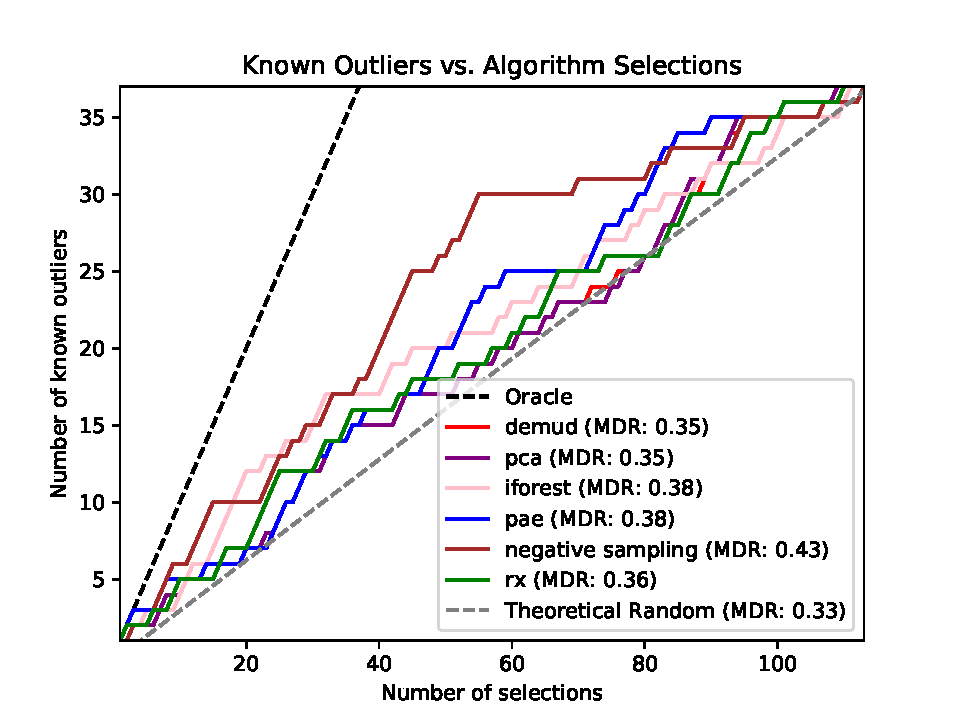
\includegraphics[width=\linewidth]{figures/faw_combined_plot.pdf}
    \caption{Number of true outliers ranked in top $N$ selections for 
    Earth science dataset.}
    \label{fig:faw_results}
\end{figure}

\begin{figure}
    \centering
    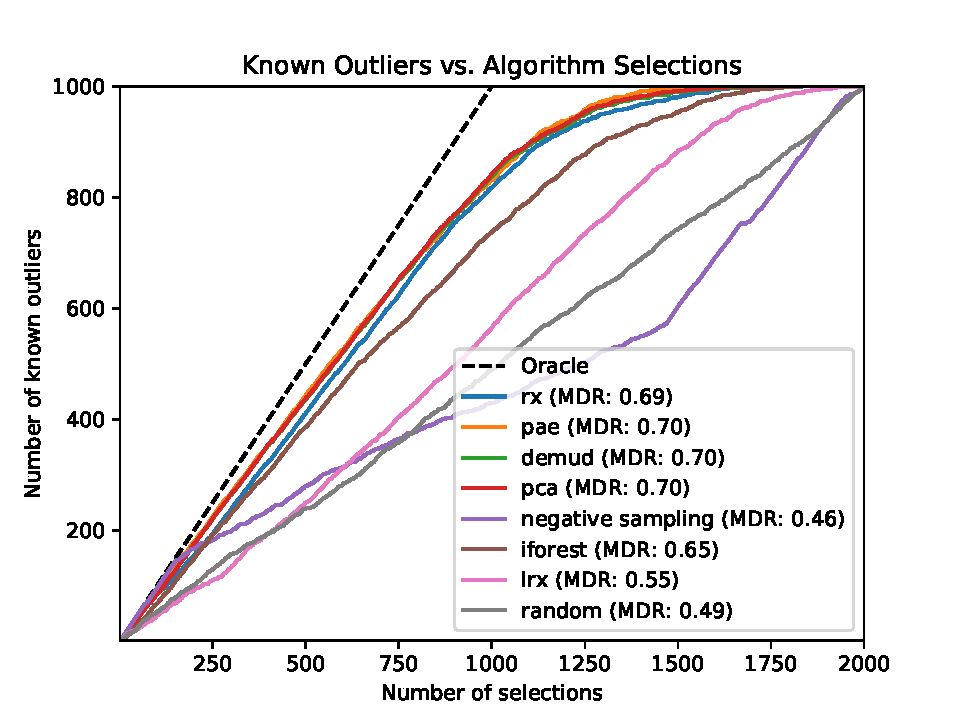
\includegraphics[width=\linewidth]{figures/fmnist_combined_plot.pdf}
    \caption{Number of true outliers ranked in top $N$ selections for 
    F-MNIST dataset.}
    \label{fig:fmnist_results}
\end{figure}

\section{Discussion}

\paragraph{Algorithm performance.} \todo{Discuss overall results from
 experiments and that we left hyperparameter tuning and extensive
 evaluation for future work.}
 
\paragraph{Evaluation in outlier detection.} \todo{Discuss why evaluation
in outlier detection applications is hard since we often don't have complete
labeled data for testing and labels can be subjective.}

\paragraph{Path to deployment.} \todo{Hannah - describe pip-installable
package, open-source for extension by the wider scientific community, etc.}

\section{Conclusions}
\todo{
Summarize conclusions and plans for future work
[Note that these datasets could also be used by other researchers as OOD
 benchmark tasks?]
 \todo{Can we make any of these datasets publicly available with the paper?}
}

\bibliography{dora_references}


\section{Acknowledgments}
We thank the NASA Center Innovation Fund and the NASA Science Mission 
Directorate (under the NASA Cross-Divisional AI Use Case Demonstration grants)
 for supporting this work.

\todo{Acknowledge DES?}
We thank the UN Food and Agriculture Organization (FAO) and Dr. Ritvik Sahajpal
(University of Maryland/NASA Harvest) for providing the fall army worm ground
 observation dataset.

We thank Raymond Francis for analyzing the Navcam rover images to
identify targets considered to be ``novel'' for evaluating outlier
detection in the planetary rover scenario.

Part of this research was carried out at the Jet Propulsion
Laboratory, California Institute of Technology, under a contract with
the National Aeronautics and Space Administration.

\end{document}

% LocalWords:  tex OOD Eigenbasis DEMUD PCA Xiaoli RX autoencoder al
% LocalWords:  Pimentel mislabeled Liang Böhm wagstaff demud Xiong
% LocalWords:  Storey Hayat des anom Lochner Chiang Zhou Liu Alvera
% LocalWords:  Azcárate Touati Prochaska Kerner kerner PyOD zhao pyod
% LocalWords:  API Umaa Vinay Navcam MNIST FashionMNIST installable
% LocalWords:  dora CIF SMD FAO Pritchard
